\chapter{Concetti di base}

\section{Introduzione}
Qui illustriamo alcuni dei concetti di base che serviranno per comprendere il resto della discussione, daremo una definizione di ontologia e tesauro, descriveremo brevemente gli strumenti utilizzati e i linguaggi con cui si descrivono le basi di conoscenza che tratteremo.

Questo capitolo non ha la pretesa di descrivere approfonditamente ogni dettaglio degli argomenti presentati, piuttosto quella di definire alcuni termini che ricorreranno frequentemente nell'elaborato, per permettere la lettura anche a chi non ha mai trattato con la rappresentazione formale della conoscenza.


\section{Basi di conoscenza}
Una base di conoscenza (Knowledge Base KB) è un insieme di affermazioni, ognuna delle quali espressa attraverso un linguaggio di rappresentazione della conoscenza. Le affermazioni esprimono concetti riguardanti il dominio di interesse.

Perché una base di conoscenza possa essere utile, deve essere possibile aggiungere conoscenza (fare affermazioni) e interrogare la KB; queste operazioni possono coinvolgere meccanismi di inferenza che permettano di ricavare nuove affermazioni da quelle già note. L'inferenza sfrutta una logica formale per ricavare nuove informazioni partendo da quelle che sono già presenti nella KB.\cite{russell2010artificial}
\subsection{Ontologie}
\subsubsection{Definizione}
In accordo con una definizione ampiamente accettata \cite{hitzler2021review} un'ontologia ha lo scopo di rappresentare un vocabolario per definire i concetti di un particolare dominio di interesse condiviso, ed è costituita da definizioni di classi, relazioni, funzioni e altri oggetti utili a rappresentare la conoscenza\cite{gruber1993translation}. 

La definizione è ancora un po' vaga, più precisamente, un'ontologia è una base di conoscenza che permette di descrivere concetti e relazioni tra di essi, specificando questi oggetti tramite un linguaggio di rappresentazione della conoscenza basato su una logica formale.
\subsubsection{Scopo delle ontologie}
Nel contesto del web semantico\footnote{Un'estensione del World Wide Web in cui le informazioni siano comprensibili a un automa\cite{berners2001new}}, le ontologie sono il mezzo principale per condividere, integrare e scoprire dati\cite{hitzler2021review}.
\subsubsection{Manipolare ontologie}
 Dato lo scopo delle ontologie, la possibilità di riutilizzare, modificare e ampliare ontologie esistenti risulta essere un argomento centrale. Spesso le basi di conoscenza sono sì strutturate, ma sono eterogenee e non permettono interoperabilità. Scopo di questo lavoro è quello di presentare degli strumenti per manipolare basi di conoscenza (ci concentriamo su tesauri e ontologie) operando in modo tale da rendere compatibili informazioni tratte da fonti differenti. 
 
 Il testo \cite{suarez2015neon} presenta una trattazione teorica approfondita sulle metodologie per sviluppare un'ontologia: in particolare il framework NeOn prevede vari scenari tipici in cui ci si può trovare quando si voglia costruire un ontologia, fa particolare attenzione ai casi nei quali siano già presenti informazioni, ma queste vanno riorganizzate.
\subsubsection{Esempio}
Consideriamo una semplice ontologia che rappresenta persone con legami di parentela genitore-figlio; le persone hanno uno o più nomi salvati nel tag \verb|comment|. Modelliamo questa ontologia con una classe \verb|Persone| e una sottoclasse \verb|Genitori| (i cui individui sono \verb|Persone| che realizzano la relazione \verb|genitoreDi|). Creiamo la relazione \verb|genitoreDi|. Infine popoliamo l'ontologia con alcuni individui. Il risultato ottenuto con Protégé è un documento XML di questo tipo:
\addxml{persone.rdf}{lst:persone.rdf}{Code/persone.rdf}
Per quanto non sia impossibile leggere la struttura e i dati dal listato precedente, un modo naturale per rappresentare le ontologie è sotto forma di grafi. Qui vediamo il grafo\footnote{Tutti i grafi presenti un questo elaborato sono stati ottenuti grazie a \url{http://vowl.visualdataweb.org/webvowl.html}} che mostra la struttura dell'ontologia e possiamo apprezzare quanto sia semplice la sua struttura rispetto a quello che avremmo potuto immaginare dal listato \ref{lst:persone.rdf}. Nel grafo non sono rappresentati gli individui, possiamo comunque leggere quanti ve ne sono per ogni classe (in questo caso un individuo di tipo \verb|Persone| e uno di tipo \verb|Genitori|)
\begin{figure}[H]
	\centering
	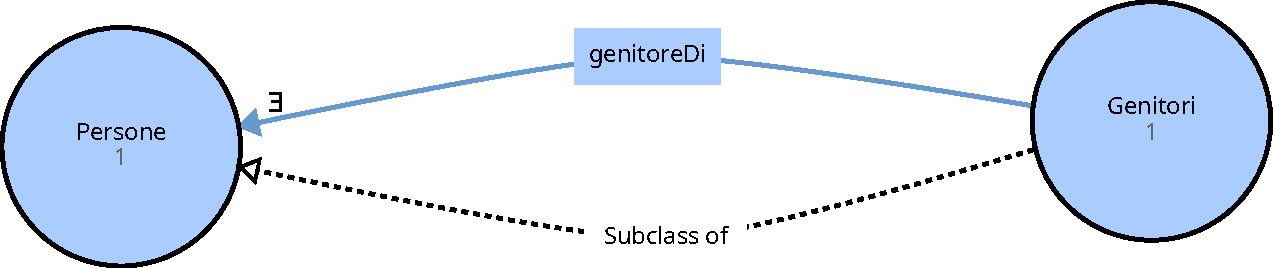
\includegraphics[width=0.5\textwidth]{Picture/persone.rdf.pdf}
	\caption{Grafo dell'ontologia persone}
\end{figure}


\subsection{Tesauri}
\subsubsection{Definizione}
Nella loro accezione più generale possibile, i tesauri sono risorse nelle quali termini affini sono raggruppati assieme\cite{kilgarriff2000s}. In particolare un tesauro fornisce un vocabolario preciso e controllato rispetto a un particolare dominio di interesse.\cite{srinivasan1992thesaurus} Queste strutture possono aiutare il ricercatore a riformulare le strategie di ricerca fornendo una serie di sinonimi, contrari, definizioni e traduzioni in altre lingue del termine cercato.

Esistono diversi tipi di tesauro in base alle modalità di costruzione e fruizione \cite{kilgarriff2000s}: nel nostro caso il tesauro sarà costituito da un vocabolario tassonomico in cui le relazioni tra oggetti sono di tipo BT (broader term), cioè ogni concetto può avere un riferimento a un concetto più generale, formando in questo modo una struttura ad albero. 
\subsubsection{Espressività}
Come si può immaginare, il potere espressivo di un tesauro è inferiore a quello di un'ontologia che non pone alcun limite alle relazioni definibili tra individui. In un tesauro inoltre ogni concetto ha, al più, un genitore, mentre in un'ontologia possiamo creare una classe che erediti le caratteristiche da più classi distinte.
\section{Strumenti di editing}

\subsection{Protégé}
Protégé\footnote{\url{https://protege.stanford.edu/}} è uno strumento per la modellazione della conoscenza molto conosciuto; è un progetto open-source sviluppato all'università di Stanford e permette la manipolazione interattiva di ontologie e KB attraverso un'interfaccia grafica e delle API java.

Le funzionalità di Protégé possono essere aumentate grazie a dei componenti plug-in il cui numero è in continua crescita. Questi plug-in offrono nuovi metodi per la gestione delle ontologie, supporto per dati multimediali, engines per il ragionamento automatico e per l'interrogazione delle basi di conoscenza\cite{sivakumar2011ontology}.
\subsubsection{Descrizione del software}
Protégé presenta un'interfaccia con numerose schede, ogni scheda permette all'utente di accedere a una differente funzionalità del software. Le schede base consentono di aggiungere nuova conoscenza e di effettuare ricerche nella KB.

Uno degli obbiettivi fondamentali di Protégé è quello di rendere l'inserimento e la ricerca in una base di conoscenza il più semplice possibile: mentre il sistema genera uno strumento per l'acquisizione della conoscenza, l'utente aggiunge informazioni riempiendo form intuitivi, selezionando elementi da liste e disegnando diagrammi.

Protégé permette di salvare le ontologie in numerosi formati, tra cui UML, XML, RDF e OWL.
\begin{figure}[h]
	\centering
	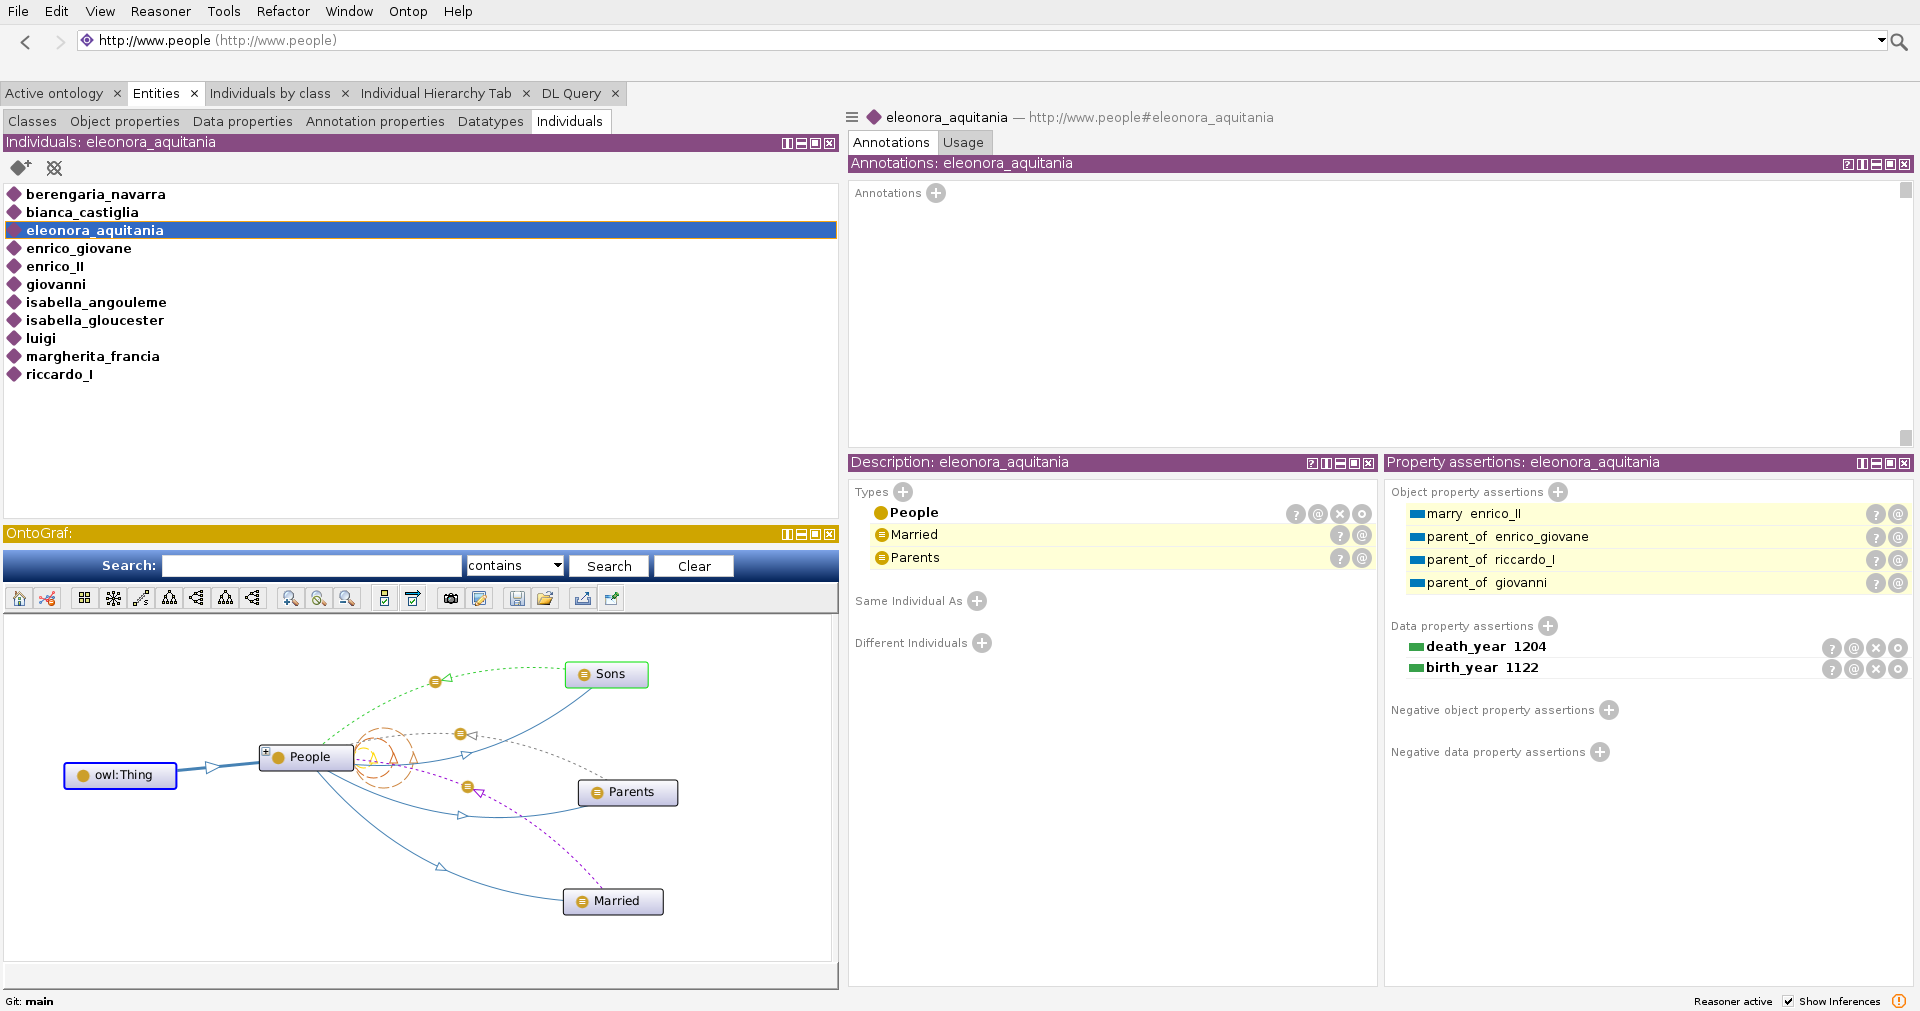
\includegraphics[width=\textwidth]{Picture/interface_protege.png}
	\caption{Interfaccia di Protégé}
\end{figure}
\subsection{\cduce}
\cduce è un linguaggio di programmazione funzionale, staticamente tipato e orientato allo sviluppo di applicazioni che lavorano su documenti XML\cite{cduceLanguage}; nasce con l'intento di migliorare XDuce, un altro linguaggio di programmazione per il processing di file XML\cite{hosoya2003xduce}. 

XDuce permette di manipolare unicamente documenti XML: questa sua specificità mostra come la presenza di feature mirate possano aiutare e semplificare lo sviluppo di applicazioni XML sacrificando, però, la possibilità di scrivere applicazioni complesse in cui non si facciano solo semplici trasformazioni di elementi XML.

\cduce si pone l'obbiettivo di integrare specifiche funzioni orientate alla manipolazione XML all'interno di un linguaggio potenzialmente general-porpouse. Per fare questo, \cduce usa un algebra general-porpouse, con costruttori di tipo standard mantenendo l'espressività e la potenza delle espressioni regolari di XDuce attraverso l'uso di tipi ricorsivi e combinatori logici (unione, intersezione, differenza).

In \cduce è possibile creare complesse strutture dati, modellare il tipo di documenti XML, e interfacciarsi in modo relativamente semplice con altri linguaggi di programmazione\cite{cduceLanguage}.
\subsection{Feature}\label{fature_cduce}
Vediamo brevemente le principali feature di \cduce, non entreremo nel dettaglio essendo presente una guida dettagliata sul sito del progetto\footnote{\url{https://www.cduce.org/}}
\subsubsection{Verifica statica dei tipi}
Il sistema di tipi è un componente centrale di \cduce; dal punto di vista pratico un tipo è un insieme di valori identificati da un'espressione sintattica: questa descrizione permette di definire in modo naturale (come insiemi matematici) relazioni di sottotipo, connettivi logici nell'algebra dei tipi ed equivalenza di tipi.

I tipi ricoprono un ruolo importante anche nella parte statica del linguaggio: la correttezza di ogni trasformazione definita in \cduce è garantita staticamente. Inoltre in \cduce il pattern matching viene effettuato attraverso un'esatta inferenza di tipo: viene assegnata a ogni variabile legata il set esatto di tutti i valori che questa può assumere.

In questo modo è possibile costruire un sistema di tipi statico e molto preciso, che permette una migliore descrizione del comportamento dinamico del programma sviluppato.
\subsubsection{Pattern matching}
\label{CDucePattern}
È un'operazione fondamentale in \cduce ed ha la forma:
\begin{minted}[tabsize=2, breaklines, bgcolor=bg]{OCaml}
match e with
	| p1 -> e1
	...
	| pn -> en
\end{minted}
Si cerca di fare il match tra la valutazione di un'espressione \verb|e| e vari pattern \verb|pi|. Il primo pattern che fa il match con \verb|e| attiva la corrispondente espressione sulla destra che può usare le variabili legate dal pattern.

Il controllo statico dei tipi assicura che il pattern matching sia esaustivo, il tipo valutato per \verb|e| deve essere sottotipo dell'unione dei tipi accettati dai pattern definiti sotto.
\subsubsection{Funzioni}
La forma generale di una funzione è
\begin{minted}[tabsize=2, breaklines, bgcolor=bg]{OCaml}
fun myfunc (t1 -> s1; ...; tn -> sn)
	| p1 -> e1
	...
	| pm -> em
\end{minted}
In cui la prima riga è l'interfaccia della funzione, il rimanente è detto corpo:
\begin{itemize}
	\item interfaccia: rappresenta il modo in cui la funzione si comporta: quando riceve un elemento di tipo \verb|ti|, la funzione restituirà un elemento di tipo \verb|si|; per ogni clausola \verb|ti -> si| il sistema verifica che la funzione trasformi correttamente gli elementi;
	\item corpo della funzione: le funzioni operano per pattern matching degli argomenti: viene eseguita la prima trasformazione tale che l'argomento ricevuto come parametro faccia il match col pattern \verb|pi|. 
\end{itemize}
In \cduce è possibile definire anche applicazioni parziali(curried functions\footnote{\url{https://en.wikipedia.org/wiki/Currying}}) e funzioni di ordine superiore\footnote{\url{https://en.wikipedia.org/wiki/Higher-order\_function}}
\section{Metalinguaggi}
Un metalinguaggio è in generale un linguaggio, o sistema di segni, naturale o artificiale, adottato per la descrizione della struttura formale di dati linguaggi\footnote{\url{https://www.treccani.it/vocabolario/metalinguaggio}}. In questo elaborato parliamo di linguaggi su tre differenti livelli:
\begin{itemize}
	\item linguaggi di programmazione: sono i linguaggi con i quali sviluppiamo strumenti più o meno automatici per la manipolazione di basi di conoscenza;
	\item ontologie e tesauri: esprimono della conoscenza in modo formale, rispettano certe logiche per poter essere usate e restituiscono all'interrogatore una risposta che quest'ultimo sia in grado di comprendere
	\item linguaggi per descrivere le basi di conoscenza: abbiamo bisogno di un linguaggio per descrivere la struttura di una KB, per definire quali relazioni possono esserci e in generale per parlare della KB stessa; chiameremo questi ultimi \say{metalinguaggi}\footnote{Questi linguaggi non ci permettono di descrivere il dominio di interesse di per sé ma descrivono come descrivere il dominio} per distinguerli dai linguaggi di programmazione e dalla conoscenza che stiamo rappresentando.
\end{itemize}
Presentiamo alcuni metalinguaggi importanti che useremo per descrivere ontologie e tesauri.
\subsection{XML}
XML (Extensible Markup Language) è un formato testuale semplice e molto flessibile, inizialmente ideato per far fronte alla pubblicazione digitale su larga scala e diventato col tempo uno strumento importantissimo per lo scambio di moltissime informazioni sul Web\cite{w3cXml}.

I documenti XML servono per memorizzare elementi detti entità che contengono dati formattati e non. I dati formattati sono costituiti da due componenti: il dato stesso e una parte di markup; quest'ultimo codifica la descrizione logica e la struttura di memorizzazione del documento. XML consente di imporre regole alla struttura logica e di memorizzazione del documento\cite{world2006extensible}.

Per una descrizione dettagliata delle specifiche di XML si rimanda a \cite{world2006extensible}, mentre \cite{li2005testing} illustra nei particolari caratteristiche e funzionalità dello Schema XML. Ci limitiamo qui a definire la struttura di un elemento XML: \verb|<(tag) (attr)>content</(tag)>| e a fornire un esempio di un'entità che potremmo trovare in un documento XML:
\begin{minted}[tabsize=2, breaklines, bgcolor=bg]{XML}
<person gender="F">
	<name>Clara</name>
	<children>
		<person gender="M">
			<name>Bob</name>
			<children/>
		</person>
	</children>
	<email>clara@lri.fr</email>
	<tel>314-1592654</tel>
</person>
\end{minted}
Questa entità descrive una donna di nome Clara, che ha un figlio maschio di nome Bob, attribuiamo a Clara anche un numero di telefono e una e-mail.

Alla luce di questa descrizione si può provare a reinterpretare il listato \ref{lst:persone.rdf} che descrive la relazione di parentela tra Giulio Cesare e Bruto.
\subsection{RDF/RDFS}
\subsubsection{RDF}
RDF (Resource Description Framework) è un framework per il processing di metadati\footnote{Esattamente come i metalinguaggi i metadati sono dati che descrivono altri dati}; un framework è un'architettura logica che supporta una prassi, una metodologia o un progetto\footnote{\url{https://it.wikipedia.org/wiki/Framework}}, in questo caso definisce le regole per la descrizione della conoscenza. RDF permette l'interoperabilità tra applicazioni che si scambiano informazioni comprensibili a un automa.

Lo scopo di RDF è quello di automatizzare il processing di risorse Web; trova quindi applicazione in: ricerca di informazioni permettendo un motore di ricerca migliore, catalogazione della conoscenza, descrizione di una collezione di pagine che rappresentano un unico \say{documento} logico, ecc...\cite{brickley1998resource}

RDF si basa sull'idea di rappresentare oggetti attraverso identificatori Web (URI\footnote{Uniform Resource Identifiers}) e di descrivere le risorse in termini di semplici proprietà e valori. I valori possono essere tipi semplici (numeri, caratteri, stringhe) oppure altre risorse identificate con URI.

RDF permette quindi di esprimere semplici affermazioni riguardo risorse attraverso grafi i cui nodi rappresentano risorse e i cui archi rappresentano proprietà e valori. Per rappresentare qualsiasi informazione in un documento RDF si usa la sintassi XML (tag e namespace)\cite{manola2004rdf}.
\subsubsection{RDFS}
Uno Schema RDF definisce quali siano le proprietà valide che si possono esprimere in una particolare descrizione con RDF; permette inoltre di imporre caratteristiche o restrizioni alle proprietà e ai valori che queste possono assumere. Per identificare uno Schema RDF viene usato il meccanismo dei namespace XML\footnote{Una serie di nomi, identificati da un URI usati in un documento XML come tipi di un elemento e nomi di attributi\cite{bray1999namespaces}}.

Interpretare uno Schema RDF significa attribuire un valore semantico a ogni proprietà presente nella descrizione RDF, questo significa che, anche se un'applicazione non è in grado di capire lo schema, può comunque ricostruire il grafo di risorse descritto da RDF\cite{miller1998introduction}.
\subsection{OWL}
L'espressività di RDF e RDFS è limitata, potendo descrivere solo predicati binari, una struttura delle classi gerarchica e proprietà anch'esse gerarchiche con un dominio e un codominio.

Sono state individuate dal gruppo di ricerca \say{Web Ontology Working Group} una serie di casi in cui le ontologie devono poter essere descritte con linguaggi più espressivi rispetto a RDF e RDFS\cite{antoniou2009web}.

Presentiamo le funzionalità aggiunte da OWL Full: la versione più espressiva\footnote{E anche più pesante computazionalmente} del linguaggio OWL; per una descrizione più approfondita del linguaggio si rimanda al documento prodotto da W3C a riguardo\footnote{\url{https://www.w3.org/TR/2004/REC-owl-features-20040210}}.
\subsubsection{OWL Full}
Presenta la compatibilità massima coi documenti RDF/RDFS, ha la massima espressività, ma non è un sistema decidibile e completo. Descriviamo questo con il solo scopo di fornire l'elenco più completo possibile di funzionalità aggiunte per aumentare l'espressività di RDF/RDFS.

OWL Full\footnote{Come anche OWL DL} permette di:
\begin{itemize}
	\item definire restrizioni sui domini delle relazioni in base alla classe (si può limitare ad esempio un individuo di classe mucca a mangiare solo piante, senza applicare la stessa restrizione ad altri animali);
	\item esprimere disgiunzione tra classi;
	\item definire classi tramite operazioni insiemistiche tra altre classi;
	\item definire restrizioni sulla cardinalità di una proprietà
	\item definire caratteristiche particolari di una proprietà come transitività, riflessività, proprietà inversa, ecc...
\end{itemize}

In OWL Full è, inoltre, possibile utilizzare ogni primitiva del linguaggio OWL combinandola con le primitive del linguaggio RDF/RDFS in modo da alterarne il significato originario (applicando anche una primitiva all'altra).
\subsection{SKOS}
SKOS (Simple Knowledge Organization System) è un modello basato su RDF che permette di esprimere la struttura base e il contenuto di schemi concettuali come tesauri, tassonomie e altri tipi di vocabolari affini\cite{isaac2009skos}.

In SKOS i concetti possono essere identificati con URI, etichettati con stringhe di caratteri in una o più lingue, descritti con delle annotazioni, associati ad altri concetti od organizzati in strutture gerarchiche informali\cite{miles2009skos}.

Più avanti vedremo che questo linguaggio è stato usato per descrivere il tesauro \say{Eurpeana Fashion Thesaurus}, questo tesauro è facilmente reperibile online ed è ottimo per i nostri esperimenti di editing (ne parleremo in \ref{ch3}).
\section{Conclusioni}
Ora che abbiamo definito i concetti base che incontreremo nell'elaborato, possiamo passare alla parte più pratica in cui vedremo come manipolare i metalinguaggi attraverso programmi in \cduce (capitolo \ref{ch2}), come la trasformazione di tag ci permetta di passare da una rappresentazione della conoscenza all'altra (capitolo \ref{ch3}) e come possiamo fare inferenza e ricavare informazioni da una base di conoscenza direttamente attraverso \cduce senza ricorrere a reasoner esterni (capitolo \ref{ch4}).